\chapter{Schnittstellen und Protokolle}
	\documentSubPartEntry{Schnittstellen und Protokolle}
	
\section{RESTfull HTTP Schnittstelle}

	\eeppi\ besitzt eine RESTfull Schnittstelle, die andere Applikationen benutzen können, um \eeppi\ direkt anzusprechen.
	Diese Schnittstelle, auch API\footnote{Cascading Style Sheets} genannt, wird auch von der eigenen Clientapplikation benutzt.

	Das API unterstützt REST\footnote{Representational State Transfer}-Level 2\footnote{REST Maturity Model: \url{http://de.wikipedia.org/wiki/Representational\_State\_Transfer\#REST\_Maturity\_Model}}.
	Das heisst, einzelne Ressourcen haben eigene Adressen
	und können unter Verwendung der HTTP-Verben GET, POST und DELETE benutzt werden.
	
\section{Dokumentation des API}
	\label{sec:apiDokumentationCreation}
	Sowohl für die Entwicklung des Clients wie auch für die weitere Entwicklung von \eeppi\ wurde das API des Servers ausführlich dokumentiert (siehe Abschnitt~\ref{sec:apiDocumentation}).
	Ein Ausschnitt der API-Dokumentation ist in Abbildung~\ref{fig:apiScreenshot} abgebildet.
	Das Konzept und die Methodik der Dokumentation wurde als Teil von \eeppi\ erstellt
	und ist strukturell an das API von Jira\footnote{\url{https://docs.atlassian.com/jira/REST/latest/}} angelehnt.
	
	\begin{figure}[H]
		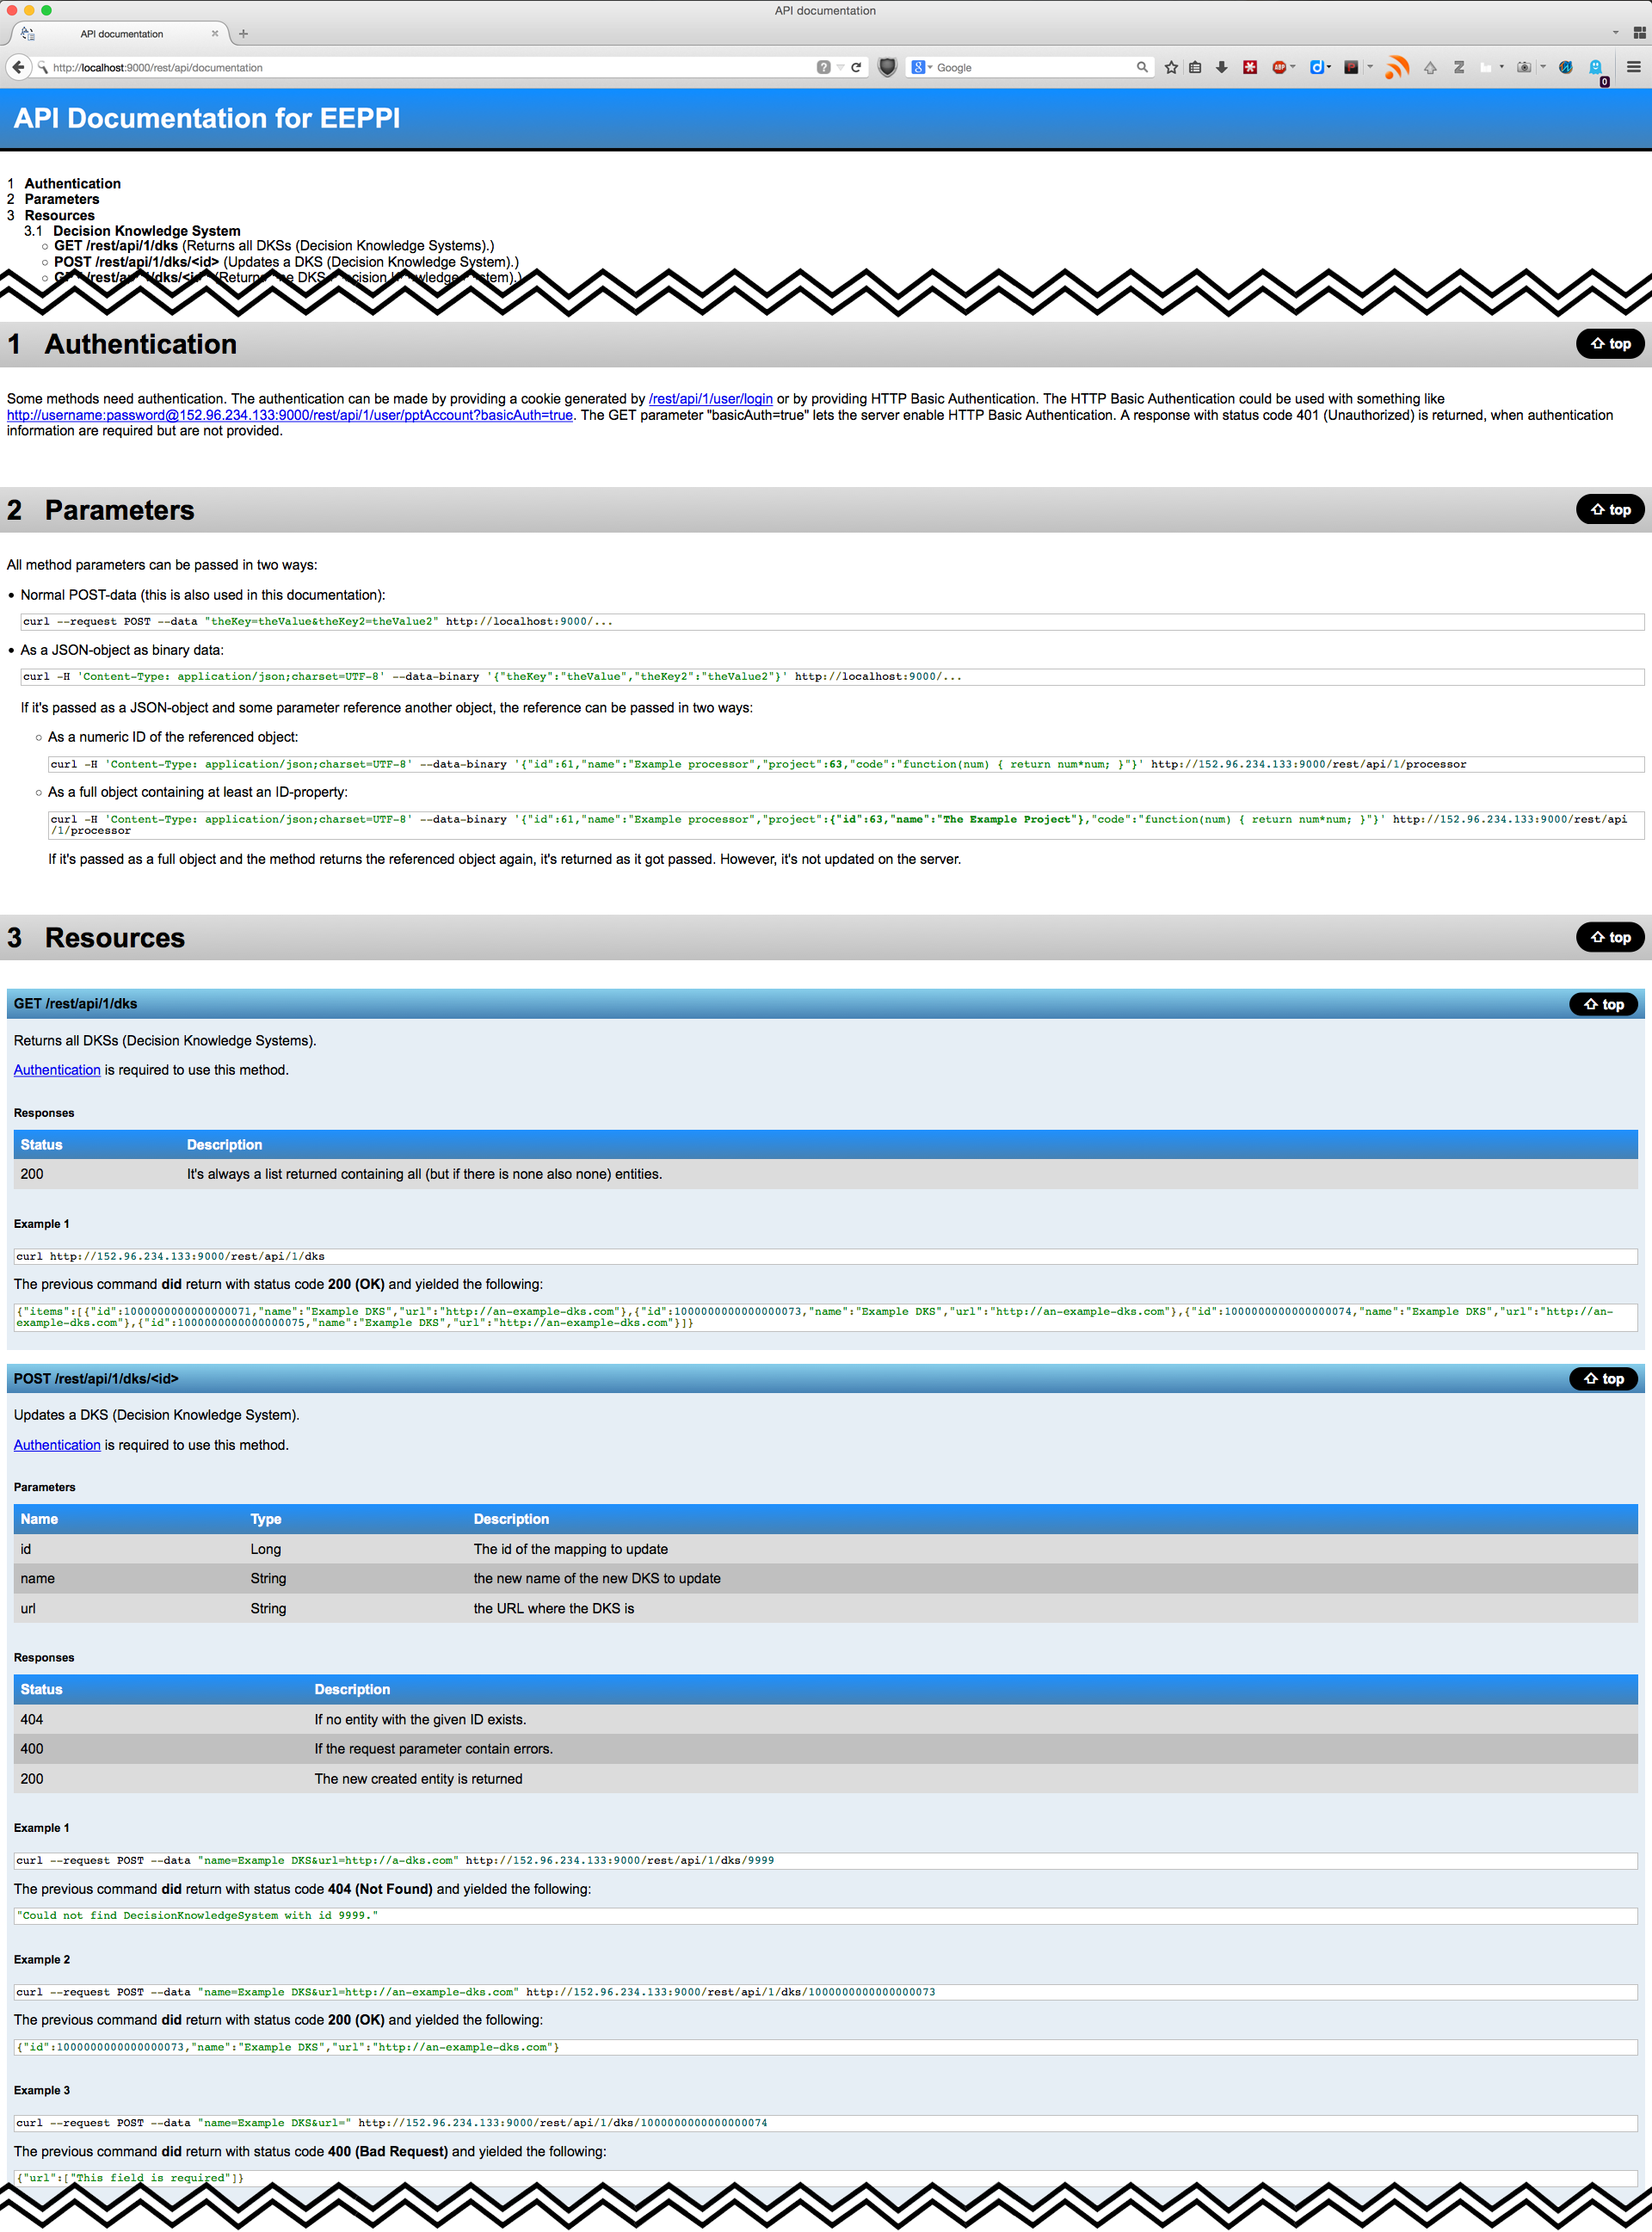
\includegraphics[width=0.9\textwidth]{interfacesAndProtocols/media/img/apiDocumentation.png}
		\centering
		\caption{API-Dokumentation im Browser (Vollständige Dokumentation siehe Abschnitt \ref{sec:apiDocumentation}) }
		\label{fig:apiScreenshot}
	\end{figure}


	\subsection{Herkunft der Daten}
		Damit das API mit möglichst geringem Aufwand jederzeit den neusten Entwicklungsstand repräsentiert, wurde darauf geachtet,
		die darin angezeigten Daten möglichst direkt aus den Originalquellen zu beziehen.
		
		
		\subsubsection{Liste aller API-Methoden}
			Die Liste der verfügbaren Methoden wird direkt aus dem Programmcode abgeleitet.
			Dazu wird mit Hilfe von Reflections\footnote{\url{http://docs.oracle.com/javase/7/docs/api/java/lang/reflect/package-summary.html}} in einem ersten Schritt die Liste aller Controller-Klassen eruiert
			und in einem zweiten Schritt deren Methoden extrahiert, die einen API-Aufruf repräsentieren.
		
		
		\subsubsection{HTTP-Verb und Pfad}
			HTTP-Verb und Ressourcenpfad werden aus der "<routes">-Datei geladen.
			Auch das Serverframework (Play Framework) lädt diese Informationen aus dieser Datei zur Delegation von Anfragen von Clients an den richtigen Controller.
			Damit ist sichergestellt, dass diese Daten in der API-Dokumentation stets aktuell sind.
			
			
		\subsubsection{Beschreibungen}
			Die verschiedenen Beschreibungen der Methoden werden aus Annotationen der Controller-Methode generiert.
			In Abbildung~\ref{fig:apiAnnotations} ist ein Beispiel eines Controllers mit Annotationen abgebildet.
			Die Annotationen beschreiben:
			\begin{itemize}
				\item{Alle Parameter}
				\item{Die Methode im Ganzen}
				\item{Dlle möglichen Rückgabestati und deren konkrete Bedeutung}
				\item{Ob eine Authentifizierung nötig ist}
				\item{Beispielaufrufe (siehe \ref{subsubsec:exampleQueries})}
			\end{itemize}
			
			\begin{figure}[H]
				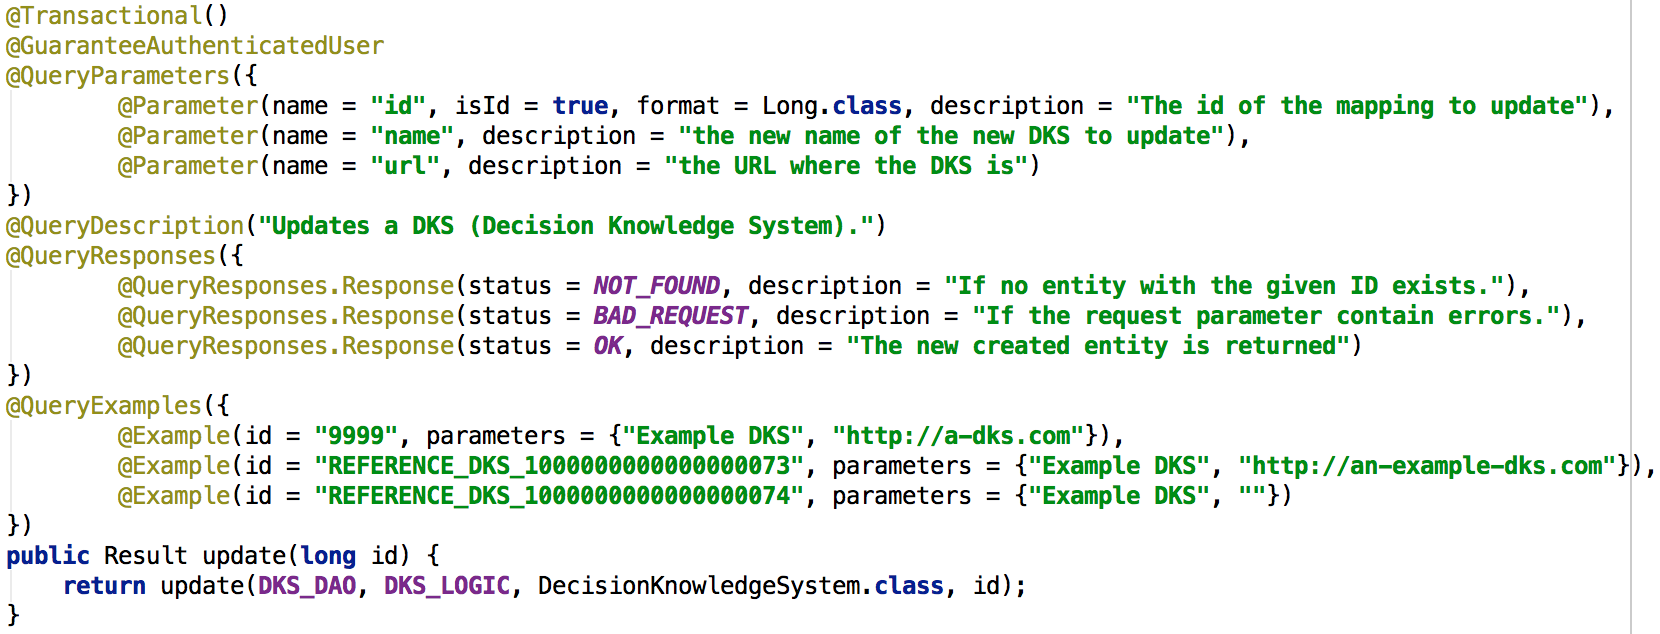
\includegraphics[width=\textwidth]{interfacesAndProtocols/media/img/apiAnnotations.png}
				\centering
				\caption{Annotations im DecisionKnowledgeSystemController}
				\label{fig:apiAnnotations}
			\end{figure}
			
			
	\subsection{Beispielaufrufe}
	\label{subsubsec:exampleQueries}
		Um dem Benutzer anzeigen zu können, dass und wie die Methode wirklich funktioniert,
		werden für jede Methode Beispielaufrufe und deren Antworten live generiert und angezeigt.
		Dazu werden bei jeder Generierung der API-Dokumentation zuerst einige Beispieldaten erstellt
		und anschliessend auf diese Daten zugegriffen über die Methoden, analog einem externen, unabhängigen Client.
		Die erhaltenen Ergebnisse werden dann in der API als "<The previous command \textbf{did} return"> angezeigt.
		Falls eine solche Simulation, beispielsweise aufgrund von externen Abhängigkeiten, nicht möglich ist,
		so ist die vom Entwickler erwartete Antwort auch in der Annotation definiert und wird dem Benutzer als
		"<The previous command \textbf{would probably} return"> angezeigt.
		
		Damit die dafür generierten Beispieldaten nicht mit den echten Daten des Systems interferieren,
		existiert für diesen Teil eine separate Datenbank.
		Diese muss der Benutzer jedoch nicht konfigurieren.
		Da die Daten nur während der Generation der API-Dokumentation benötigt werden
		und nicht längerfristig persistiert werden müssen,
		werden sie lediglich in einer SQLite-Datenbank\footnote{Einfache Datenbank, in welcher die Daten in einer einzigen Datei gespeichert werden} gespeichert.
	


\section{Client}
		Die \eeppi\ Clientapplikation nutzt die RESTfull Schnittstelle zum Datenaustausch mit dem Server sowie zur Kommunikation mit Remote-Hosts über den Proxy (Cross-Original Aufruf).
		
		Um auf dem Client einfach und flexibel Prototypen aus übertragenen JSON-Objekten instanziieren zu können, gibt es eine Object Factory.
		Diese baut anhand einer Factorykonfiguration, die jedes übertragbare Objekt deklarieren muss, Objekte zusammen und füllt sie mit Daten.
		Diese zusätzliche Konfiguration ist notwendig, da JavaScript nicht genügend Typeninformationen besitzt, aus denen sich die erforderlichen Informationen ermitteln liessen und TypeScript diese nicht automatisch generieren kann.
		Alternativ liesse sich die Prototypeninstanziierung  durch Factoryfunktionen pro Objekt umsetzen, dies hat sich jedoch während der Entwicklung als wartungsintensiv und Duplicated-Code-lastig erwiesen.
		
		
\section{HTTP Verben}
		RESTfull impliziert die Verwendung der richtigen Verwendung der HTTP Verben: 
		\begin{description}
			\item[GET] für Abfragen
			\item[POST] für Create-Operationen
			\item[DELETE] für Lösch-Operationen
			\item[PUT oder POST] für Update-Operationen.
		\end{description}
		
		Viele Netzwerkadministratoren erlauben PUT und DELETE nicht und blockieren entsprechenden Verkehr. Aus diesem Grund setzen Entwickler häufig nur GET und POST ein.
		
		Wir haben uns entschieden, serverseitig beides zu ermöglichen:
		Um Objekte zu löschen kann entweder 'DELETE /<entity>' oder 'POST /<entity>/delete' aufgerufen werden.
		
		Die Client Applikation verwendet nur POST und GET, dies kann allerdings umkonfiguriert werden.
		PUT Requests werden von \eeppi\ in der Standardkonfiguration gar nicht verwendet,
		es kommt stattdessen immer POST zum Einsatz.
